\section{Results}
\label{sec:results}

\begin{table*}[t]
\centering
\caption{Every scenario on the same $50$ paired evaluation seeds, one
simulator and one $42$-decision measurement window. Where uplink OFDMA is
enabled the scheduler is service-period aligned and the sleep guard is
disabled, so no row depends on that workaround. The hand-designed controller
is tuned on disjoint seeds under a service floor; the row marked
\emph{free choice} lets that search pick its own OFDMA mode, and it picks
off. Learned rows give the mean and standard deviation over $10$ training
seeds. The last three columns compare each learned method against the
\emph{free choice} controller at $166.5$\,J, Wilcoxon signed-rank:
\emph{mean over runs} averages the ten fits per seed; \emph{oracle}
is each method's lowest-energy fit, selected on the same evaluation seeds
it is scored on, and is therefore retrospective. \emph{backlog} is a
drain-time proxy, per-station queue bytes over that station's offered
rate, averaged over stations and decisions; it is not a measured packet
latency. $>$3\,s is the fraction of decisions whose mean proxy exceeds
three seconds. OFDMA: share of decisions with the scheduler enabled.}
\label{tab:main}
\footnotesize
\setlength{\tabcolsep}{4.5pt}
\begin{tabular}{lrrrrrrrr}
\toprule
 & & & & & & \multicolumn{2}{c}{mean over runs} & oracle \\
\cmidrule(lr){7-8}\cmidrule(lr){9-9}
Scenario & $E$ (J) & tput (Mb/s) & backlog (ms) & $>$3\,s & OFDMA & $\Delta$ vs hand & $p$ & $\Delta$ vs hand \\
\midrule
No TWT, no OFDMA & $441.1$ & $24.95$ & $2637$ & $0.24$ & $0\,\%$ & & & \\
Static TWT & $173.3$ & $21.03$ & $2789$ & $0.37$ & $0\,\%$ & & & \\
Static TWT $+$ OFDMA & $282.2$ & $19.82$ & $2823$ & $0.40$ & $100\,\%$ & & & \\
Random TWT & $171.1$ & $14.47$ & $3159$ & $0.63$ & $0\,\%$ & & & \\
Random TWT $+$ OFDMA & $228.5$ & $13.51$ & $3188$ & $0.66$ & $100\,\%$ & & & \\
OFDMA only, no TWT & $477.8$ & $24.30$ & $2652$ & $0.25$ & $100\,\%$ & & & \\
Random joint action & $198.8$ & $14.29$ & $3157$ & $0.63$ & $48\,\%$ & & & \\
Hand-designed, OFDMA on & $265.5$ & $18.37$ & $2904$ & $0.43$ & $100\,\%$ & & & \\
Hand-designed, \emph{free choice} & $166.5$ & $19.22$ & $2888$ & $0.41$ & $0\,\%$ & & & \\
\midrule
\multicolumn{9}{l}{\emph{offline RL, 10 training seeds each}} \\
\quad IQL & $107.3 \pm 2.6$ & $20.76$ & $2805$ & $0.38$ & $0\,\%$ & $-35.6\,\%$ & $10^{-15}$ & $-37.2\,\%$ \\
\quad DQN$+$CQL & $193.0 \pm 10.1$ & $20.54$ & $2829$ & $0.40$ & $23\,\%$ & $+15.9\,\%$ & $10^{-5}$ & $+1.6\,\%$ \\
\quad Dueling$+$CQL & $194.1 \pm 14.7$ & $20.49$ & $2834$ & $0.40$ & $25\,\%$ & $+16.6\,\%$ & $10^{-6}$ & $+0.7\,\%$ \\
\quad DDQN & $222.7 \pm 13.5$ & $15.64$ & $3076$ & $0.58$ & $43\,\%$ & $+33.8\,\%$ & $10^{-15}$ & $+23.7\,\%$ \\
\quad BC & $255.1 \pm 12.4$ & $19.78$ & $2875$ & $0.43$ & $48\,\%$ & $+53.2\,\%$ & $10^{-15}$ & $+42.7\,\%$ \\
\bottomrule
\end{tabular}
\end{table*}


\subsection{The two mechanisms do not combine}

Table~\ref{tab:main} holds three pairs differing only in the OFDMA bit, and in
each enabling it costs energy: $+62.8\,\%$ under the static schedule,
$+33.6\,\%$ under random TWT, $+8.3\,\%$ with TWT off.

Throughput falls in all three, so this is not a throughput-for-energy trade.

The ordering is the informative part: the penalty is largest where TWT sleeps
hardest and smallest where it does not sleep at all, because soliciting a
station competes with the schedule trying to keep it asleep.

\subsection{The cost is carrier sensing, not lost sleep}

Our first explanation was that triggers wake sleeping stations. The traces
refute it. Mean sleep occupancy---the fraction of the control window a station
spends in PHY sleep, averaged over the sixteen---differs by under $0.8$
percentage points between the OFDMA arms. Stations sleep just as much; their
awake time simply costs more.

Per-state traces from a separate instrumented run---the tuned controller with
and without the scheduler, which differ by $113.7$\,J there---place $69\,\%$
of the extra energy in carrier-sense busy and $24\,\%$ in receive, $9\,\%$ in
transmit, against $-1\,\%$ in idle. A solicited station is awake across the
trigger, its own transmission and the acknowledgement, and the awake portion
outside its own transmission is charged at the CCA-busy current.

The scenario leaves CCA-busy at ns-3's default $273$\,mA against its own
$66$\,mA receive current---an internally inconsistent parameterisation---so we
re-evaluated every load-bearing arm at $66$\,mA, same policies and seeds.
Energies fall $21$--$27\,\%$ unevenly, but both conclusions hold: OFDMA costs
$+57.8\,\%$ rather than $+62.8\,\%$ under the static schedule, and IQL beats
the controller by $31.2\,\%$ ($84.6$ against $123.1$\,J) rather than
$35.6\,\%$. Signs survive the power profile; magnitudes do not.

\subsection{One algorithm beats the tuned rule}

Given a free choice the tuned controller disables OFDMA, worth $99$\,J
($265.5$ against $166.5$\,J); we take that stronger form as the baseline.


IQL reaches $107.3 \pm 2.6$\,J, the spread being the standard deviation over
ten training runs, not a confidence interval. That is a $35.6\,\%$ reduction;
the interval $[-36.5,-34.7]\,\%$ is a paired bootstrap over the fifty shared
seeds of the per-seed mean across runs, and $p = 1.8\times10^{-15}$ is a
two-sided Wilcoxon signed-rank test on the same pairing. Neither propagates
uncertainty from resampling training runs; the across-run spread is reported
separately. The reduction comes with higher
mean throughput, $20.76$ against $19.22$\,Mb/s, and a backlog proxy lower by
$83$\,ms ($p = 9.8\times10^{-9}$ paired); the change in the fraction of
decisions above three seconds is not statistically detectable ($p = 0.07$). Its worst fit of ten,
$112.4$\,J, still beats every other method's best.

That column is a drain-time proxy---queue bytes over offered rate---not a
measured latency, so it tracks standing backlog: flat across all $42$ decisions,
$2.6$--$2.9$\,s where throughput stays near offered load and $3.1$--$3.2$\,s
where it does not. We use it as a guard against starving traffic, not as a
latency claim.

\subsection{Four of five do not, and selection is why}

Table~\ref{tab:main} is why we claim this for IQL and not for offline RL as a
family. The \emph{mean over runs} column averages the ten fits per evaluation
seed, estimating expected performance over training randomness: DQN$+$CQL is
$15.9\,\%$ worse than the hand-designed rule ($p = 8.6\times10^{-5}$),
dueling DQN$+$CQL $16.6\,\%$ worse ($p = 4.3\times10^{-6}$), DDQN and
behaviour cloning worse still.

The \emph{oracle} column takes each method's lowest-energy fit, chosen on the
same seeds it is then scored on. There the CQL variants sit within $1.6\,\%$ of
the baseline with no difference detected ($p = 0.74$, $0.55$)---a failure to
detect, not evidence of equivalence, under retrospective selection. The gap
between the columns is what matters: expected performance over training
randomness is $16\,\%$ worse than a hand-written rule, while a retrospectively
chosen fit is not distinguishable from it. Whether an off-policy estimator can
pick that fit in advance across independent runs is open; we validate FQE only
for ranking checkpoints within a run.

IQL is the exception because it barely varies: its across-fit standard deviation
is $2.6$\,J against $10.1$ to $14.7$\,J for the others, so which fit you deploy
does not matter.

\begin{figure}[t]
  \centering
  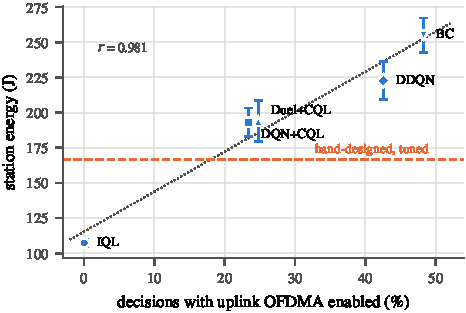
\includegraphics[width=\columnwidth]{figures/fig_ordering.pdf}
  \caption{Station energy against how often each learned policy enables uplink
  OFDMA; bars are the standard deviation over ten training runs. The association
  across these five algorithm-level means is strong ($r = 0.981$, $n=5$) but
  descriptive: the methods differ in schedule and grouping too. Dashed: the
  tuned controller.}
  \label{fig:ordering}
\end{figure}

\subsection{What separates the methods is the OFDMA bit}

The five methods order by energy as they order by how often they enable the
scheduler (Fig.~\ref{fig:ordering}), from IQL at $0\,\%$ to behaviour cloning
at $48\,\%$---the last because the logger chose the bit by coin flip and
imitating it reproduces that.

The lowest-energy method is the one that disables the scheduler, and the
coordinate search reaches the same configuration independently. The obvious objection is that we crippled the scheduler: ns-3 solicits four
stations per trigger by default, while schedule~11 leaves eight awake and the
channel admits nine resource units, so half the awake set was unreachable.
Raising the limit to nine makes uplink OFDMA worse, not better---$+87.4\,\%$
against the no-OFDMA arm instead of $+62.8\,\%$ under the static schedule, and
$+83.3\,\%$ instead of $+59.5\,\%$ for the hand-designed controller, both
$+15\,\%$ on the default at $p = 2\times10^{-15}$ with throughput falling at
each step. Solicitation cost scales with the stations a trigger names; the
benefit scales with the data they have, and in this mix they have little.

Each seed either holds its offered load constant or steps it by $1.5$ to
$2.5\times$ partway through. Splitting the fifty on that flag gives $35.1\,\%$
below the baseline on the $19$ constant-load seeds ($p = 3.8\times10^{-6}$) and
$35.8\,\%$ on the $31$ stepped ones ($p = 9.3\times10^{-10}$): robustness to
within-distribution load variation, not transfer to unseen traffic.

\subsection{Is the adaptation necessary?}

IQL and the tuned controller both disable uplink OFDMA, so the gap between them
cannot come from that bit. Would one well-chosen fixed configuration do as
well? We swept all $20$ schedules at the deployed grouping on the tuning seeds
with OFDMA off, picked the Pareto-efficient ones from tuning data alone, and
evaluated those on the untouched evaluation seeds.

None matches IQL. At its energy the best fixed schedule delivers
$12.62$\,Mb/s against $20.76$---$64\,\%$ more data for the same power, with the
energy difference undetectable ($p = 0.12$); at its throughput the best fixed
schedule costs $179.1$\,J against $107.3$, so IQL is $40\,\%$ cheaper. One
schedule is beaten on both axes at once ($145.4$\,J, $17.93$\,Mb/s), and on the
tuning seeds no schedule of the twenty comes within $10\,\%$ of IQL's energy at
$90\,\%$ of its throughput.

The traces say why. IQL uses $14.9$ distinct actions per $42$-decision
episode, and the schedules it favours are poor alone: schedule~18 for
$43\,\%$ of decisions and schedule~19 for $23\,\%$ deliver $15.64$ and
$12.74$\,Mb/s as fixed policies. Holding either costs about what IQL costs
while moving a third less data, so the gain is in moving between schedules, not
in any one. We swept schedules at the deployed grouping only, so this is the
best fixed \emph{schedule}, not the best of all $380$ configurations.

\subsection{Validation}

Four instrumentation faults materially affected earlier evaluations, each
invisible in aggregate statistics: a convergence gate that discarded a sound
checkpoint ranking ($6.5\,\%$ energy); a saturated reward energy term
($13.3$\,J, though the unrepaired reward still beat the baseline by
$27.5\,\%$); two harnesses whose measurement windows differ by a warm-up; and
an $8$\,ms sleep deferral applied only with the OFDMA bit set, worth
$+62.0\,\%$ alone---two thirds of a penalty we had charged to the protocol,
and one that moved sleep \emph{occupancy} under $0.8\,\%$.
